\documentclass{minimal}
\usepackage{tikz}

\begin{document}
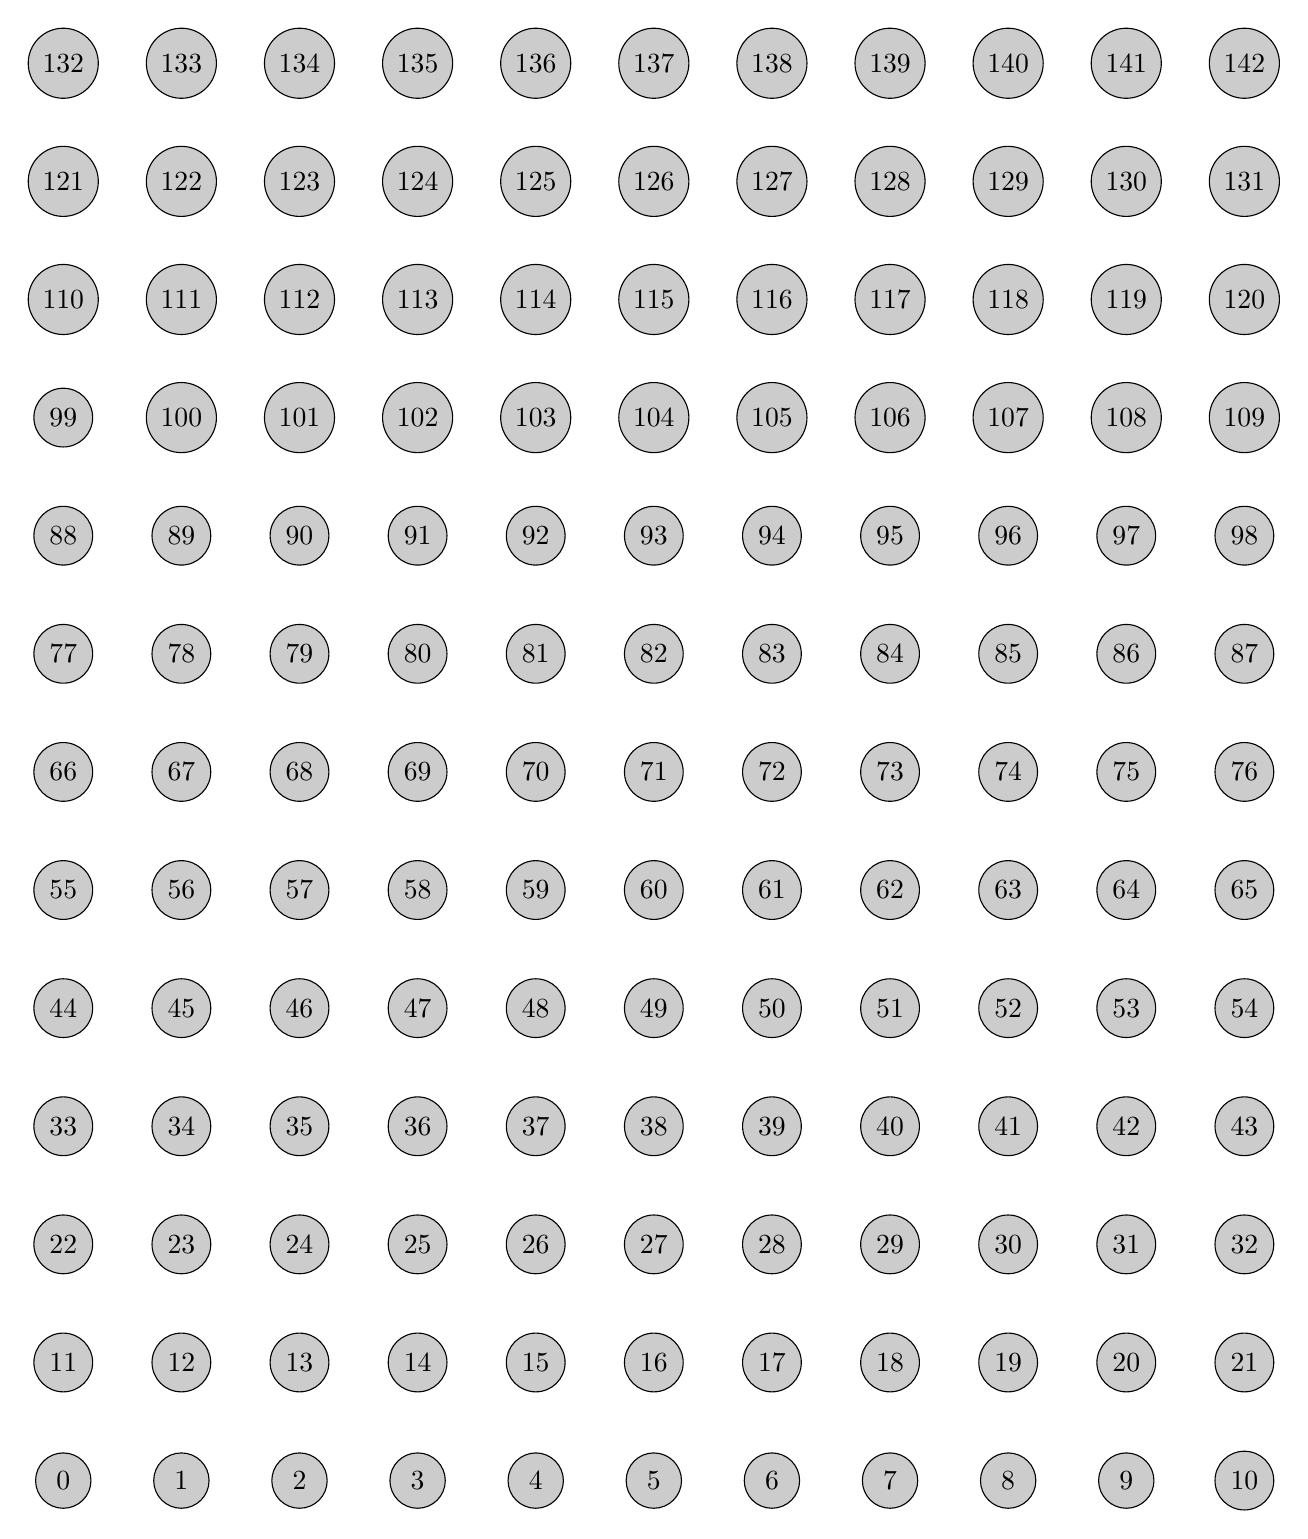
\begin{tikzpicture}[darkstyle/.style={circle,draw,fill=gray!40,minimum size=20}]
  \foreach \x in {0,...,10}
    \foreach \y in {0,...,12} 
       {\pgfmathtruncatemacro{\label}{\x + \y *11}
       \node [darkstyle]  (\x\y) at (1.5*\x,1.5*\y) {\label};} 

\end{tikzpicture}
\end{document}
